\section{Softwarearchitektur und Design}

\begin{concept}{Überblick Softwareentwicklung}\\
Die Entwicklung von Software erfolgt in verschiedenen Ebenen:
\begin{itemize}
    \item Business Analyse (Domänenmodell, Requirements)
    \item Architektur (Logische Struktur)
    \item Entwicklung (Konkrete Umsetzung)
\end{itemize}
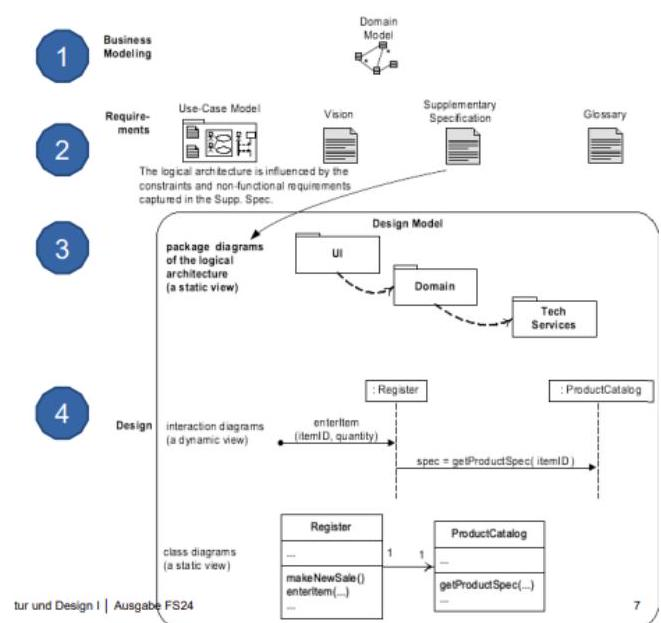
\includegraphics[width=0.9\linewidth]{images/2024_12_29_0d1d7b5551ea1b4b41bdg-07(2)}
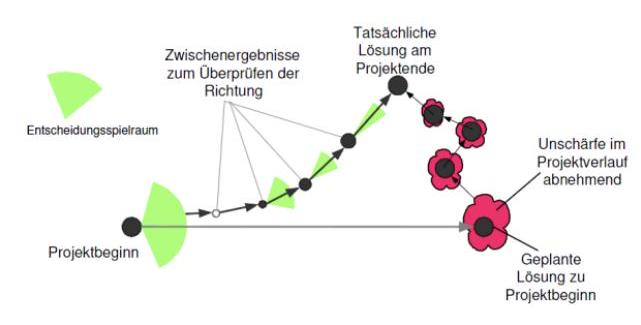
\includegraphics[width=0.9\linewidth]{images/2024_12_29_0d1d7b5551ea1b4b41bdg-08(1)}
\end{concept}

\begin{definition}{Softwarearchitektur}\\
Die Architektur definiert:
\begin{itemize}
    \item Grundlegende Strukturen und Komponenten
    \item Heutige und zukünftige Anforderungen
    \item Weiterentwicklungsmöglichkeiten
    \item Beziehungen zur Umgebung
\end{itemize}
\end{definition}

\begin{concept}{Architekturanalyse}\\
Die Analyse erfolgt iterativ mit den Anforderungen:
\begin{itemize}
    \item Analyse funktionaler und nicht-funktionaler Anforderungen
    \item Abstimmung mit Stakeholdern
    \item Kontinuierliche Weiterentwicklung
\end{itemize}
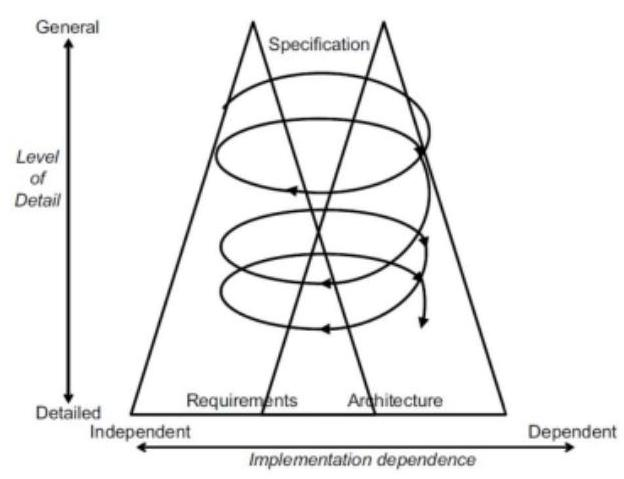
\includegraphics[width=0.9\linewidth]{images/2024_12_29_0d1d7b5551ea1b4b41bdg-08}
\end{concept}

\begin{theorem}{ISO 25010 vs FURPS+}\\
\textbf{ISO 25010:}
\begin{itemize}
    \item Hierarchische Struktur für nicht-funktionale Anforderungen
    \item Definierte Hauptcharakteristiken und Subcharakteristiken
    \item Messbare Metriken für jede Anforderung
    \item Präzise Formulierung und Verifikation
\end{itemize}

\textbf{FURPS+:}
\begin{itemize}
    \item Functionality (Funktionalität)
    \item Usability (Benutzbarkeit)
    \item Reliability (Zuverlässigkeit)
    \item Performance (Leistung)
    \item Supportability (Wartbarkeit)
    \item + (Implementation, Interface, Operations, Packaging, Legal)
\end{itemize}
\end{theorem}

\begin{concept}{Modulkonzept}\\
Ein Modul (Baustein, Komponente) wird bewertet nach:
\begin{itemize}
    \item \textbf{Kohäsion:} Innerer Zusammenhang
    \item \textbf{Kopplung:} Externe Abhängigkeiten
\end{itemize}

\textbf{Eigenschaften:}
\begin{itemize}
    \item Autarkes Teilsystem
    \item Minimale externe Schnittstellen
    \item Enthält alle benötigten Funktionen/Daten
    \item Verschiedene Formen: Paket, Library, Service
\end{itemize}
\end{concept}

\begin{concept}{Architektursichten}\\
Das N+1 View Model beschreibt verschiedene Perspektiven:
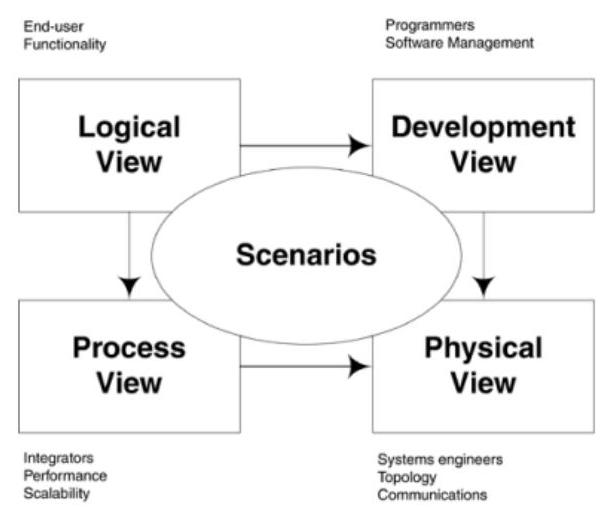
\includegraphics[width=0.9\linewidth]{images/2024_12_29_0d1d7b5551ea1b4b41bdg-09}

\textbf{UML-Paketdiagramm:}
\begin{itemize}
    \item Definition von Teilsystemen
    \item Gruppierung von Elementen
    \item Abhängigkeiten zwischen Paketen
\end{itemize}
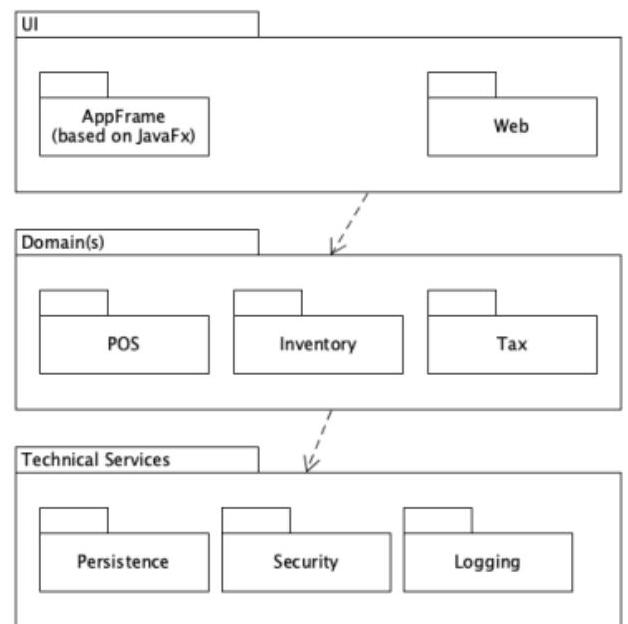
\includegraphics[width=0.9\linewidth]{images/2024_12_29_0d1d7b5551ea1b4b41bdg-09(1)}
\end{concept}

\subsubsection{UML-Modellierung}

\begin{KR}{Statische vs. Dynamische Modelle}\\
\textbf{Statische Modelle (Struktur):}
\begin{itemize}
    \item UML-Klassendiagramm
    \item Fokus auf Pakete, Klassen, Attribute
    \item Keine Methodenimplementierung
\end{itemize}

\textbf{Dynamische Modelle (Verhalten):}
\begin{itemize}
    \item UML-Interaktionsdiagramme
    \item Fokus auf Logik und Verhalten
    \item Implementierung der Methoden
\end{itemize}
\end{KR}

\begin{definition}{UML-Diagrammtypen}\\
\textbf{1. Klassendiagramm:}
\begin{itemize}
    \item Klassen und aktive Klassen
    \item Attribute und Operationen
    \item Sichtbarkeiten und Beziehungen
    \item Interfaces und Realisierungen
\end{itemize}

\textbf{2. Sequenzdiagramm:}
\begin{itemize}
    \item Lebenslinien und Nachrichten
    \item Synchrone/Asynchrone Kommunikation
    \item Aktivierung und Deaktivierung
    \item Alternative Abläufe
\end{itemize}

\textbf{3. Zustandsdiagramm:}
\begin{itemize}
    \item Zustände und Übergänge
    \item Start- und Endzustände
    \item Composite States
    \item Historie und Parallelität
\end{itemize}

\textbf{4. Aktivitätsdiagramm:}
\begin{itemize}
    \item Aktionen und Aktivitäten
    \item Kontroll- und Datenflüsse
    \item Verzweigungen und Zusammenführungen
    \item Partitionen (Swimlanes)
\end{itemize}
\end{definition}

\begin{concept}{Responsibility Driven Design (RDD)}\\
Design basierend auf Verantwortlichkeiten:
\begin{itemize}
    \item Klassenentwurf nach Rollen
    \item Kollaborationsbeziehungen
    \item Implementierung durch Attribute/Methoden
    \item Anwendbar auf allen Ebenen
\end{itemize}
\end{concept}

\begin{theorem}{GRASP Prinzipien}\\
General Responsibility Assignment Software Patterns:
\begin{itemize}
    \item \textbf{Information Expert:} Verantwortung basierend auf Information
    \item \textbf{Creator:} Objekterstellung bei starker Beziehung
    \item \textbf{Controller:} Zentrale Steuerungslogik
    \item \textbf{Low Coupling:} Minimale Abhängigkeiten
    \item \textbf{High Cohesion:} Starker innerer Zusammenhang
    \item \textbf{Polymorphism:} Flexibilität durch Schnittstellen
    \item \textbf{Pure Fabrication:} Künstliche Klassen für besseres Design
    \item \textbf{Indirection:} Vermittler für Flexibilität
    \item \textbf{Protected Variations:} Kapselung von Änderungen
\end{itemize}
\end{theorem}

\begin{example}{Architekturentwurf}
\textbf{Aufgabe:} Entwerfen Sie die grundlegende Architektur für ein Online-Banking-System.

\textbf{Lösung:}
\begin{itemize}
    \item \textbf{Anforderungsanalyse:}
    \begin{itemize}
        \item Sicherheit (ISO 25010)
        \item Performance (FURPS+)
        \item Skalierbarkeit
    \end{itemize}
    
    \item \textbf{Architekturentscheidungen:}
    \begin{itemize}
        \item Mehrschichtige Architektur
        \item Microservices für Skalierbarkeit
        \item Sicherheitsschicht
    \end{itemize}
    
    \item \textbf{Module:}
    \begin{itemize}
        \item Authentifizierung
        \item Transaktionen
        \item Kontoführung
    \end{itemize}
\end{itemize}
\end{example}

\begin{KR}{Architekturentwurf}
\textbf{Schritte:}
\begin{enumerate}
    \item Anforderungen analysieren
    \item Architekturstil wählen
    \item Module identifizieren
    \item Schnittstellen definieren
    \item Mit Stakeholdern abstimmen
\end{enumerate}

\textbf{Qualitätskriterien:}
\begin{itemize}
    \item Änderbarkeit
    \item Wartbarkeit
    \item Erweiterbarkeit
    \item Testbarkeit
\end{itemize}
\end{KR}